% Document class report-template accepts either: project-plan or final-report option
\documentclass[final-report]{report-template}

% Packages I want to use in my report.
\usepackage{graphicx}
\usepackage{subfigure}
\usepackage{amsmath}
\usepackage{blindtext}
\usepackage{listings}
\usepackage{lmodern}

% \def\LOGO{%
% \begin{picture}(0,0)\unitlength=1cm
% \put (3,-1) {\includegraphics[width=5em]{school_badge.png}}
% \end{picture}
% }

% Define and Set the code part style
\lstdefinestyle{mystyle}{
    backgroundcolor=\color{backcolour},   
    commentstyle=\color{blue!20!black!50!green},
    keywordstyle=\color{blue!70},
    numberstyle=\tiny\color{codegray},
    stringstyle=\color{codepurple},
    basicstyle=\footnotesize,
    breakatwhitespace=false,         
    breaklines=true,                 
    captionpos=b,                    
    keepspaces=true,                 
    numbers=left,                    
    numbersep=5pt,                  
    showspaces=false,                
    showstringspaces=false,
    showtabs=false,                  
    tabsize=2
}
\lstset{style=mystyle, escapeinside=``}


% Directory where I save my figures.
\graphicspath{{./figures/}}

% \university{Imperial College London}
% \department{Department of Earth Science and Engineering}
% \course{MSc in Applied Computational Science and Engineering}
% \title{Forecasting induced seismicity in Oklahoma}
% \author{Zhiyong Liu}
% \email{zl1220@ic.ac.uk}
% \githubusername{acse-liuzyon}
% \supervisors{Dr. Stephen P. Hicks}
\repository{https://github.com/acse-2020/acse2020-acse9-finalreport-liuzyon}


\begin{document}

\begin{titlepage}

\newcommand{\HRule}{\rule{\linewidth}{0.5mm}} % Defines a new command for the horizontal lines, change thickness here

\center % Center everything on the page

%----------------------------------------------------------------------------------------
%	HEADING SECTIONS
%----------------------------------------------------------------------------------------

\textsc{\LARGE Imperial College London}\\[1.5cm] % Name of your university/college
\textsc{\Large Department of Earth Science and Engineering}\\[0.5cm] % Major heading such as course name
\textsc{\large MSc in Applied Computational Science and Engineering}\\[0.5cm] % Minor heading such as course title

%----------------------------------------------------------------------------------------
%	TITLE SECTION
%----------------------------------------------------------------------------------------

\HRule \\[0.4cm]
{ \huge \bfseries Forecasting induced seismicity in Oklahoma}\\[0.4cm] % Title of your document
\HRule \\[1.5cm]
%----------------------------------------------------------------------------------------
%	AUTHOR SECTION
%----------------------------------------------------------------------------------------

\begin{minipage}{0.4\textwidth}
    \begin{flushleft} \large
    \emph{Author:}\\
    Zhiyong \textsc{Liu}\\ % Your name
    zl1220@ic.ac.uk\\
    Github: acse-liuzyon
    \end{flushleft}
    \end{minipage}
    ~
    \begin{minipage}{0.4\textwidth}
    \begin{flushright} \large
    \emph{Supervisor:} \\
    Dr. Stephen P. \textsc{Hicks}\\ % Supervisor's Name
    s.hicks@imperial.ac.uk
    \end{flushright}
\end{minipage}\\[2cm]

%----------------------------------------------------------------------------------------
%	LOGO SECTION
%----------------------------------------------------------------------------------------


\includegraphics[width=0.4\textwidth]{school.png}\\[4cm] % Include a department/university logo - this will require the graphicx package
 
%----------------------------------------------------------------------------------------


%----------------------------------------------------------------------------------------
%	DATE SECTION
%----------------------------------------------------------------------------------------

{\large \today}\\[2cm] % Date, change the \today to a set date if you want to be precise


\vfill % Fill the rest of the page with whitespace

\end{titlepage}


% Metadata used for the title page.

% \maketitlepage  % generate title page
\githubrepo  % GitHub repository

% Abstract
\section*{Abstract}
Human activities can cause minor earthquakes, which changes the stresses and strains on the earth's crust.
These earthquakes are called induced earthquakes and most have a low magnitude. 
Multi-year research by the United States Geological Survey (USGS) published in 2015 showed that most of large earthquakes occured in Oklahoma may have been caused by deep injection of wastewater from the oil industry.
In this project, a unique and rich dataset of industrial activities from regions in Oklahoma are used and correlations between these activities and seismicity are confirmed.
With existing high-quality earthquake catalogues in these regions, possible signatures of human-induced seismicity are retrospectively forecasted through machine learning techniques. 
At the end of the project, a working forecasting model is generated and tested the permormance by the test dataset splitted from total dataset.

\textbf{Key Words:} induced earthquakes, machine learning method, forecasting model
\newpage

% Introduction section
\section{Introduction}
It is well known that humans can cause earthquakes through fluid injection and extraction. Ellsworth stated the understanding of the causes and mechanics of human-induced earthquakes. It includes wastewater injection, emerging oil and gas recovery technologies, and other indirect induced activities,
including deep fluid injection \citep{ellsworth2013injection}.
Norbeck and Rubinstein genreated a model based on fluid flow and seismic physics, which associate the past injection trends with the seismicity patterns \citep{norbeck2018hydromechanical}.
Such cases of induced seismicity have been recorded and proven in Oklahoma, where seismicity has been increased dramatically since 2010.
In cases like Oklahoma, because the rate of earthquakes was very low before high-rate wastewater injection, it is relatively easy to determine the fundamental causes of induced seismicity.
Therefore, due to the low background stress in intraplate regions, the human triggering signatures are clearly identifiable.
However, in tectonically-active areas, it is more challenging to distinfuish between natural and triggered seismicity.
In tectonically active regions in the US, such as California, although oil and gas extraction has taken place for many decades, only a handful of studies have been published with a focus on these areas \citep{Hough2017WasTM}. 
Big-data and statistical approaches will be crucial in separating natural causes from potential human triggering factors in these areas.
In regions from Oklahoma, Hincks et al. developed a Bayesian network to for quantitative evaulation of correlations between well operational parameters, geological formation, and seismicity.
The injection depth relative to crystalline basement was found to be the most significant parameter for seismic moment release \citep{hincks2018oklahoma}.
Also, Wozniakowska and Eaton performed a machine learning estimation of the seismogenic activation potential for each well using logistic regression and also found that the injection depth influence greatly the seismogenic activation potential \citep{wozniakowska2020machine}.

The correlations of induced earthquakes with fluid injection activities are well established, even in previous research some physics models are also developed for earthquake prediction.
It is still not known why some areas are more susceptible to induced earthquakes.
In this project, Several unique and rich datasets of industrial activities from regions in Oklahoma are used to statistically evaluate and retropectively forecast possible signatures of human-induced seismicity from existing high-quality earthquake in these regions. 
These datasets contains geological formation, injections, hydraulic fracturing activities and wells, which all have millions of items.
They were selected subset from 2011 to 2018 and displayed on the local map of Oklahoma. Rough visual correlations between the earthquakes and these potential induced factors were discovered.
Then, stepwise regression method was used to choose statistically significant features from all features. A logistic model was fitted before and after stepwise regression, which proved that the work of features selection indeed benefit to induced forecasting. 

In previous studies for induced earthquakes in Oklahoma, forecasting works were almost always implemented using regression models. Compared to them, after selecting statistically significant features, this project originally designed and implemented a neural network for induced seismicity forecasting, which effectively improves the performance of model fitting and prediction. 

\begin{figure}
    \begin{center}
        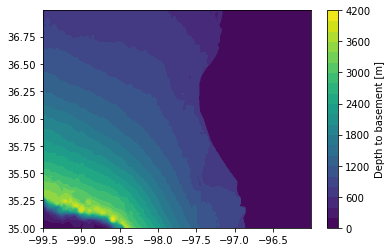
\includegraphics[width=0.5\textwidth]{depth_to_basement.png}
    \end{center}
    \caption{\label{fig:depth_to_basement} Depth to basement in Oklahoma.}
\end{figure}

\begin{figure}
    \begin{center}
        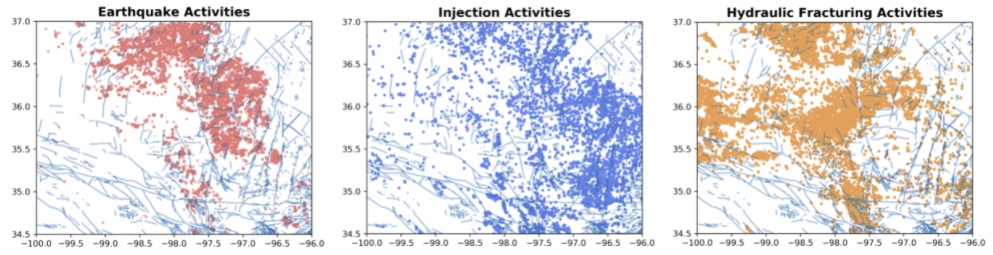
\includegraphics[width=1\textwidth]{activity.png}
    \end{center}
    \caption{\label{fig:activity} Activities during 2011 to 2018 in interest area from Oklahoma.}
\end{figure}

% Another section
\section{Software Description}
\subsection{Visualization: Matplotlib \& GeoPandas}
GeoPandas can help researcher make working with geospatial data in Python easier. It extends the datatypes in Pandas, which allows users perform spatial operations on geometric types.
Matplotlib is a comprehensive library for creating static, animated, and interactive visualizations in Python.
In the initial phase of project, we visualized the geological formation (depth to basement) and the various activities (seismicity, injection, hydraulic fracturing) in interest area on the Oklahoma map by GeoPandas and Matplotlib as shown in Fig~\ref{fig:depth_to_basement} and Fig~\ref{fig:activity}.
By comparing these pictures, we found a rough spatial correlation between them.
\subsection{Stepwise Regression}
In any phenomenon, some factors will play a more important role in determining the outcome. Stepwise Regression is method which is widely used to find which factors are important and which are not. 
The factors that have a rather high p-value do not make a meaningful contribution to the accuracy of our predictions. 
Therefore, only the important factors are retained to ensure that the model make predictions based on the factors that will help it produce the most accurate results.

P-values are often used to see if the patterns they measured were statistically significant. If the p-value of a statistical test is small enough, we are able to reject the null hpytothesis of the test and the pattern measured is statistically significant.
The most common threshold for p is 0.05. For the variable whose p-value is greater than 0.05, we can assume that it is not statistically significant as shown in Fig~\ref{fig:p-value}. Here is step in stepwise logistic regression process.
The `injection\_vol', `HF\_Base\_Water\_Volume', `HF\_Base\_NoWater\_Volume' both have a p-value than threshold 0.05 in logistic regression results, which are not statistically significant and should be eliminated in later process.

\begin{figure}
    \begin{center}
        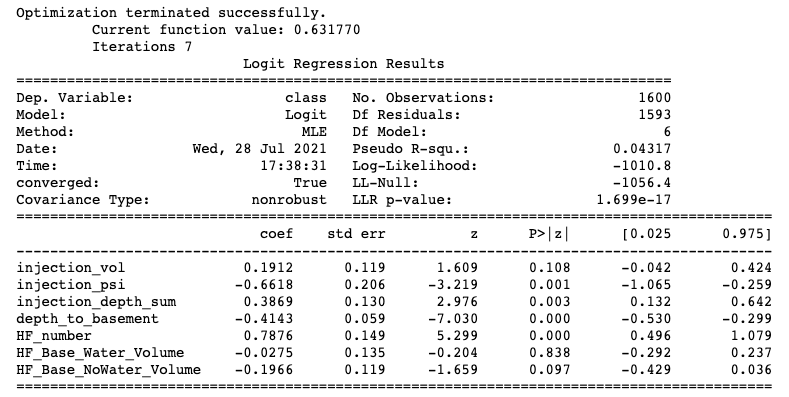
\includegraphics[width=0.8\textwidth]{p-value.png}
    \end{center}
    \caption{\label{fig:p-value} Activities during 2011 to 2018 in interest area from Oklahoma.}
\end{figure}

In this project, we performed a stepwise logistic regression that used a backwards elimination approach on all interest potential factors \citep{Ryan}.
All factors were initially included and the least statistically significant factor is eliminated in each step. In other words, the most 'useless' factor is dropped. This process continued untill all factors kept are statistically important.

\subsection{Neural Network Construction: Pytorch}
Pytorch is an open source machine learning library for Python and is completely based on Torch library,
used for applications such as computer vision and natural language processing. It is mostly developed by Facebook's AI Research lab (FAIR) \citep{patel2018two}. 
PyTorch provides two features:
\begin{itemize}
    \item Tensor computing (like Numpy) with strong acceleration via graphics processing units (GPU)
    \item Deep neural networks built on a type-based automatic differentiation system.
  \end{itemize}
Pytorch provides a class called Tensor (torch.Tensor) to store and operate on homogeneous multidimensional rectangular arrays of numbers. 
They are tailored for datasets in machine learning. Tensors in Pytorch are similar to Numpy Arrays, but it supports to be operated on a CUDA-capable Nvidia GPU \citep{paszke2019pytorch}.

To define a neural network in Pytorch, it is pretty convenient to create a class that inherits from nn.Module as below:
\begin{lstlisting}[language=Python]
    # Get cpu or gpu device for training.
    device = "cuda" if torch.cuda.is_available() else "cpu"
    print("Using {} device".format(device))
    
    # Define model
    class NeuralNetwork(nn.Module):
        def __init__(self):
            super(NeuralNetwork, self).__init__()
            self.flatten = nn.Flatten()
            self.linear_relu_stack = nn.Sequential(
                nn.Linear(4, 8),
                nn.ReLU(),
                nn.Linear(8, 8),
                nn.ReLU(),
                nn.Linear(8, 2),
                nn.ReLU()
            )
    
        def forward(self, x):
            x = self.flatten(x)
            logits = self.linear_relu_stack(x)
            return logits
    
    model = NeuralNetwork().to(device)
\end{lstlisting}
User can define the layers of the network in the \textit{\_\_init\_\_} function and indicates how data will pass through the network in the \textit{forward} function. 
With Pytorch, user can move it to the GPU to accelate operations in the neural netwok if available. Figure~\ref{fig:neural_network_example} is the model created above trained on the playground online through Tensorflow. 
The neural network prediction model used in this project is implemented by this way.
\begin{figure}
    \begin{center}
        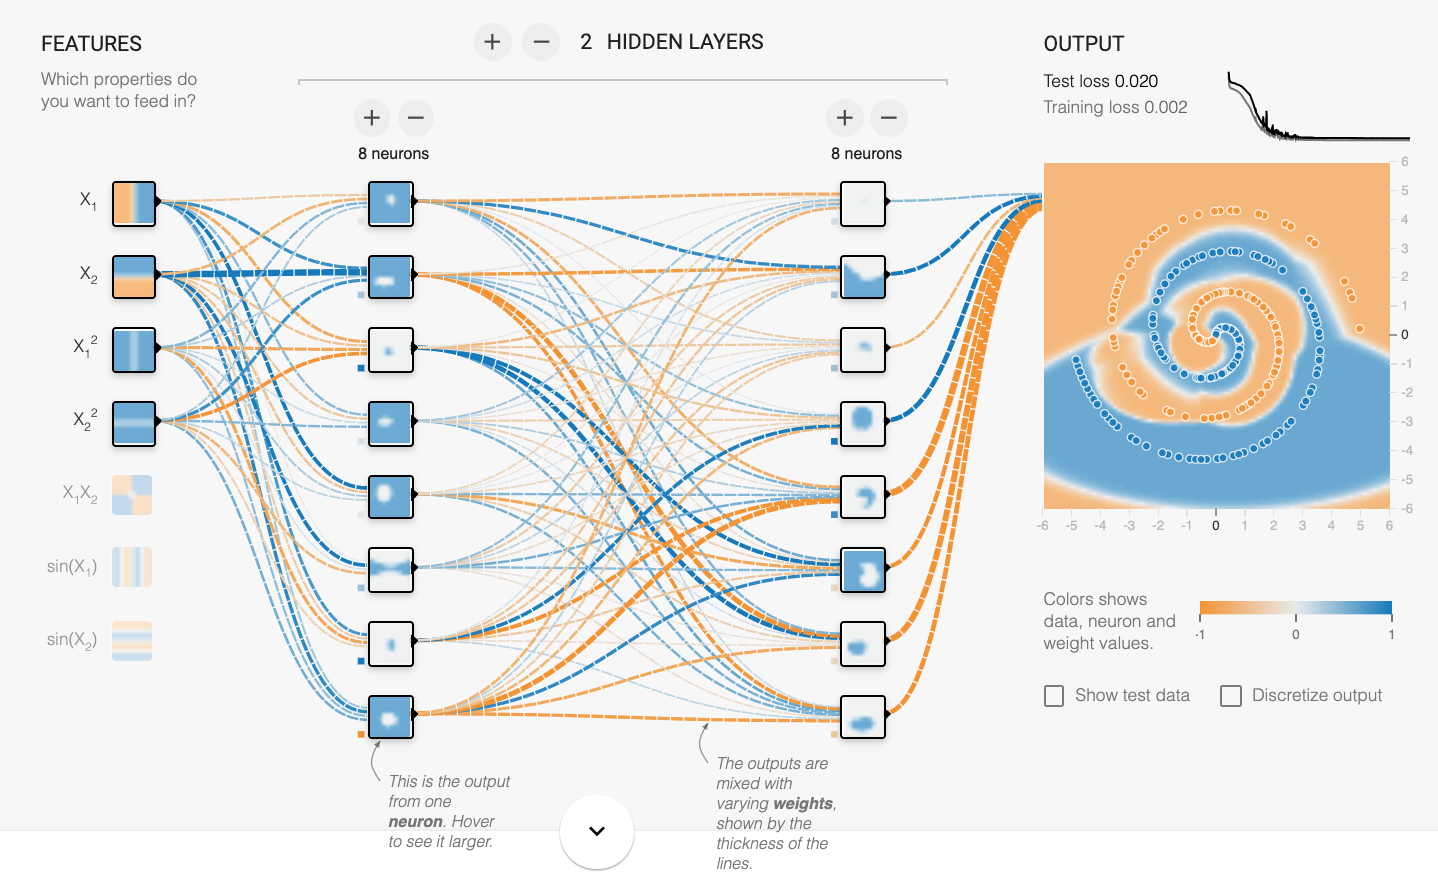
\includegraphics[width=1\textwidth]{neural_network_exmaple.png}
    \end{center}
    \caption{\label{fig:neural_network_example} The model created simulated in playground.tensorflow.org}
\end{figure}

\subsection{Feature Attribution: Captum}
Feature attribution is the technique to investgiate how much each feature in the model contributes to the prediction for given dataset fitting. 
With the increase in model complexity and the resulting lack of transparency, model interpretability methods have become increasingly important in machine learning field.
In this project, we implemented a neural network model with the PyTorch library \citep{PyTorch} for improving the accuracy of prediction. Therefore, we use the Captum for feature attribution in neural network model, which is a model interpretability and understanding library for Pytorch.
It includes general purpose implementations of integrated gradients, saliency maps, smoothgrad, vargrad and others for PyTorch models.

Captum provides advanced algorithms, including Intergarated gradientes used in this project, to provides users an simple way to understand which features are contributing to a models' output.
Integrated gradients represents the integral of gradients with respect to inputs along the path from a given baseline to input. The integral can be approximated using a Riemann Sum or Gauss Legendre quadrature rule. Formally, it can be described as follows in Equation \eqref{equ:inreGrad}:

\begin{figure}
    \begin{center}
        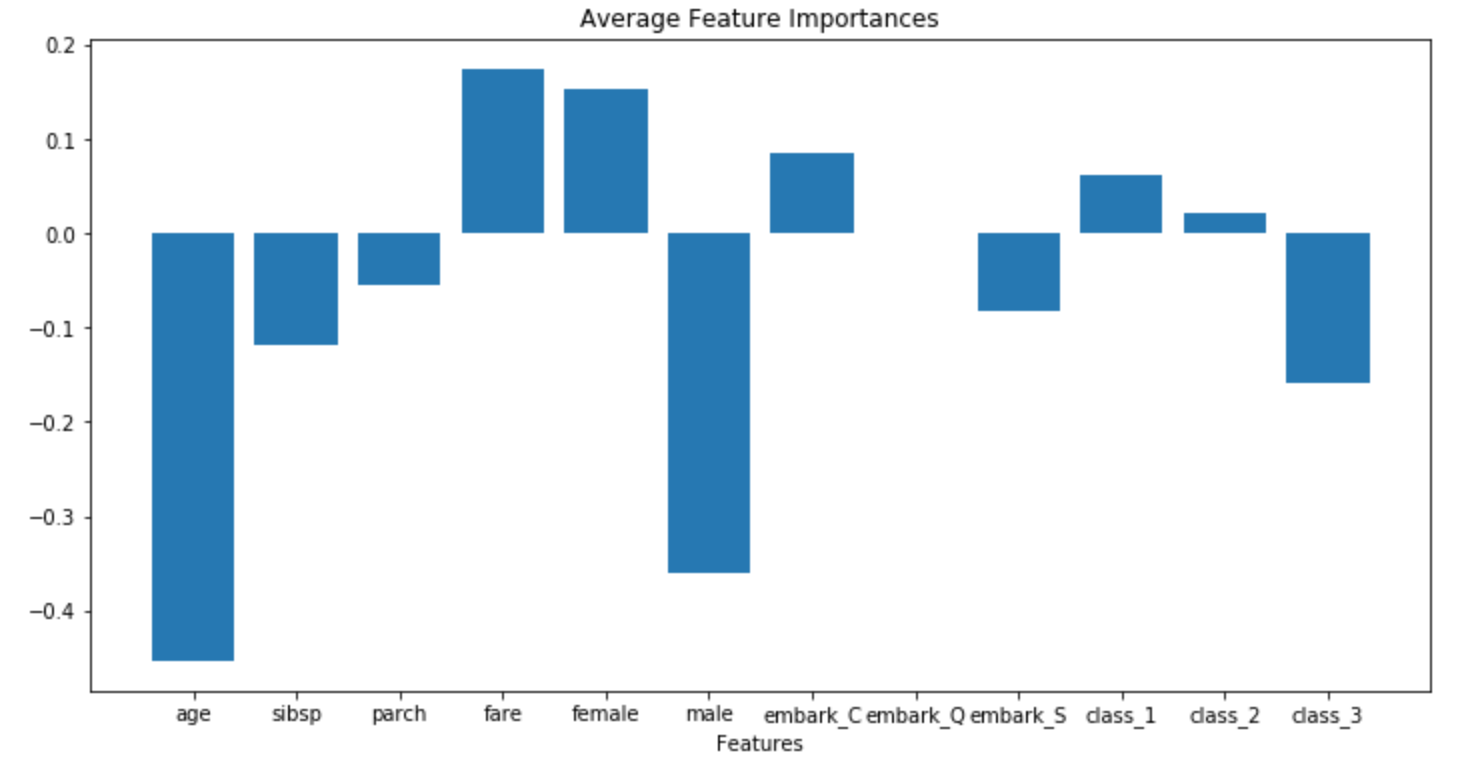
\includegraphics[width=0.8\textwidth]{feature_importance.png}
    \end{center}
    \caption{\label{fig:feature_importance} Feature Importance Example in Captum Tutorial.}
\end{figure}

\begin{equation}
    IntegratedGrads_{i}(x) ::= (x_{i} - x_{i}^{'}) \times 	\int_{\alpha=0}^1 \frac{\partial F(x^{'}+\alpha \times (x-x^{'}))}{\partial x_{i}} d\alpha  \label{equ:inreGrad}    
\end{equation}

Intergarated Gradients along the i-th dimension of input X. Alpha is the scaling coffecient \citep{sundararajan2017axiomatic}.

As shown in Fig~\ref{fig:feature_importance}, this is the result of feature importance analysis for the model trained in official tutorial of Captum.
The official tutorial used an example model trained on the titanic survival data. 
It first trained a deep neural network on the data using Pytorch and used Captum to understand which of the features were most important and how the network reached its prediction.
The features involved Age, Sibsp, Parch, Fare, Gender, Embark, Class and the target is a binary indicating whether passager is survived. After normalization and one-hot encodings, the neural network architecture was defined and trained. 
The neural network had a simple architecture using 2 hidden layers, the first with 12 hidden units and the second with 8 hidden units, each with Sigmoid non-linearity.
The final layer performed a softmax operation and had 2 units, corresponding to the outputs of either survived or not survived. The accuracy of this model on dataset achieved to $81.6\%$. To perform feature attribution on this model, this example applied integrated Gradients, which is one of the Feature Attribution methods included in Captum. The feature attribution method code is shown in below.

\begin{lstlisting}[language=Python]
    ig = IntegratedGradients(model)
    test_input_tensor.requires_grad_()
    attr, delta = ig.attribute(test_input_tensor,target=1, return_convergence_delta=True)
    attr = attr.detach().numpy()

    # Helper method to print importances and visualize distribution
    def visualize_importances(feature_names, importances, title="Average Feature Importances", plot=True, axis_title="Features"):
        print(title)
        for i in range(len(feature_names)):
            print(feature_names[i], ": ", '%.3f'%(importances[i]))
        x_pos = (np.arange(len(feature_names)))
        if plot:
            plt.figure(figsize=(12,6))
            plt.bar(x_pos, importances, align='center')
            plt.xticks(x_pos, feature_names, wrap=True)
            plt.xlabel(axis_title)
            plt.title(title)
    visualize_importances(feature_names, np.mean(attr, axis=0))
\end{lstlisting}

The result of feature attribution was listed in Table~\ref{tab:feature_importance} and shown in Fig~\ref{fig:feature_importance}.
From the feature attribution information, we obtain some interesting insights regarding the importance of various features. We see that the strongest features appear to be age and being male, which are negatively correlated with survival. Embarking at Queenstown and the number of parents / children appear to be less important features generally.

\begin{table}[]
    \caption{Average Feature Importances for each feature}
    \label{tab:feature_importance}
    \resizebox{\textwidth}{6mm}{
    \begin{tabular}{|c|c|c|c|c|c|c|c|c|c|c|}
    \hline
    age    & sibsp  & parch  & fare  & male   & embark\_C & embark\_Q & embark\_S & class\_1 & class\_2 & class\_3 \\ \hline
    -0.454 & -0.119 & -0.056 & 0.175 & -0.359 & 0.086     & -0.001    & -0.082    & 0.062    & 0.021    & -0.159   \\ \hline
    \end{tabular}}
    \end{table}

% \section*{Conclusions}

% References
\bibliographystyle{agsm}
\bibliography{references.bib}  % BibTeX references are saved in references.bib

\end{document}          

